\section{Scheduling e operazioni sui processi}
Si ritiene necessario dare un nome alle attività compiute dalla CPU: in particolare, i sistemi \textbf{batch} eseguono \textbf{job}, mentre quelli \textbf{time-sharing} dei \textbf{task}. Chiamiamo queste attività col nome generale di \textbf{processo}.\par
Intuitivamente, un processo è un programma in esecuzione il cui stato è rappresentato da program counter e registri del processore. Si compone di: \begin{itemize}
	\item \textbf{Sezione di testo}: Contiene il codice eseguibile.
	\item \textbf{Sezione dei dati}: Contiene le variabili globali.
	\item \textbf{Heap}: Memoria allocata dinamicamente durante l'esecuzione del programma.
	\item \textbf{Stack}: Memoria usata temporaneamente nelle chiamate a funzione.
\end{itemize}
\noindent È importante notare che heap e stack sono di dimensione variabile e crescono l'una verso l'altra; è compito del sistema operativo garantire che non si sovrappongano. La prima aumenta o diminuisce di dimensione grazie a funzioni come malloc e free per il linguaggio C, mentre le chiamate a funzione inseriscono un \textbf{record} di attivazione contenente parametri, variabili locali e indirizzo di ritorno sulla stack, per poi rimuoverlo quando il controllo del programma ritorna al chiamante.\par
Noi sappiamo che un programma diventa processo quando il suo eseguibile è caricato in memoria e sebbene due processi possono essere associati ad uno stesso programma, sono da considerare come due istanze diverse, le quali seguono il proprio percorso di esecuzione, detto \textbf{thread}. Inoltre, durante la loro vita, i processi possono presentarsi nei seguenti stati: \begin{itemize}
	\item \textbf{Nuovo}: Il processo è appena creato.
	\item \textbf{In esecuzione}: Le istruzioni del processo stanno venendo eseguite.
	\item \textbf{In attesa}: Il processo attende il verificarsi di un evento.
	\item \textbf{Pronto}: Il processo attende di essere assegnato a un'unità di elaborazione.
	\item \textbf{Terminato}: Il processo ha terminato l'esecuzione.
\end{itemize}
\noindent Questi stati sono comuni a tutti i sistemi operativi, sebbene alcuni introducano ulteriori distinzioni. È bene inoltre notare che sebbene più processi possano essere pronti, i core delle unità di elaborazione possono eseguirne solo uno per volta.
\begin{figure}[h]
	\centering
	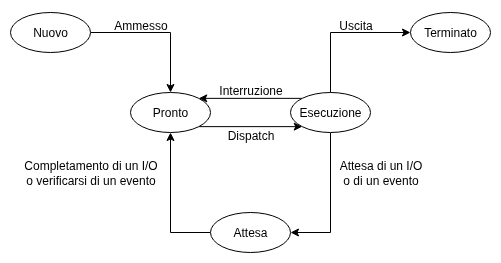
\includegraphics[width=0.8\linewidth]{Images/FSM_processes.png}
	\caption{Diagramma degli stati di un processo}
\end{figure}

\noindent Nei sistemi operativi i processi si rappresentano con \textbf{blocchi di controllo} (Process Control Block, PCB), depositi di informazioni per ogni processo specifico. Salvano dati in merito allo stato corrente, il valore del program counter, lo stato dei registri della CPU e informazioni sul suo scheduling, informazioni sulla gestione della memoria, di accounting e infine sullo stato dell'I/O.\par
Nei sistemi operativi moderni si è esteso il concetto di processo introducendo la possibilità di avere più percorsi di esecuzione, permettendo ai processi di svolgere più compiti alla volta. In un sistema che supporta i thread, infatti, il PCB è esteso per includere informazioni su di essi.\newline

\noindent Riprendiamo ora il concetto di \textbf{multiprogrammazione}, il cui obiettivo è avere almeno un processo sempre in esecuzione per massimizzare l'utilizzo della CPU. Il cambio tra i vari processi avviene così frequentemente da consentire l'interazione con ciascun programma durante la loro esecuzione ed è gestita dallo \textbf{scheduler}, il quale seleziona il processo e lo assegna al core della CPU. Le architetture odierne comprendono CPU a più core, ed in particolare chiamiamo \textbf{grado di multiprogrammazione} il numero di processi in memoria in un dato istante.\par
Il bilanciamento tra multiprogrammazione e time sharing richiede di tener conto anche del comportamento complessivo dei processi: definiamo infatti \textbf{I/O-bound} i processi che impiegano la maggior parte del tempo nell'esecuzione di operazioni input/output e \textbf{CPU-bound} quelli che eseguono nella maggior parte elaborazioni. Ogni processo è inizialmente inserito dallo scheduler in una \textbf{coda dei processi pronti}, tipicamente implementata come una struttura dati, in attesa di essere assegnato ad un core. Esiste inoltre una \textbf{coda di attesa} dove sono spostati i processi in attesa del completamento di un evento, come la ricezione di un input.
\begin{figure}[h]
	\centering
	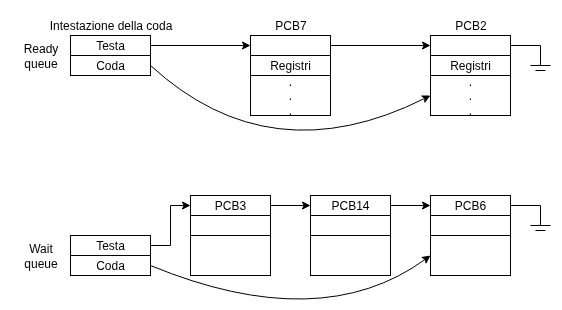
\includegraphics[width=1\linewidth]{Images/ready-wait_queues.png}
	\caption{Coda dei processi pronti e di attesa}
\end{figure}

\noindent Con l'inserimento nella coda dei processi pronti, si possono verificare i seguenti casi: \begin{itemize}
	\item Processo emette richiesta I/O, viene spostato quindi nella coda di I/O.
	\item Processo crea un processo figlio, attendendo la sua terminazione.
	\item Processo rimosso forzatamente dalla CPU a causa di interruzione. Viene reinserito nella coda dei processi pronti.
\end{itemize}
\noindent Nei primi due casi, al completamento della richiesta I/O o al termine del processo figlio, il processo originale passa dallo stato di attesa a quello pronto ed è nuovamente inserito nella coda dei processi pronti. Il ciclo continua fino al termine dell'esecuzione e si rimuoverà quindi da tutte le code, deallocando anche il PCB e le risorse legate al processo.
\begin{figure}[h]
	\centering
	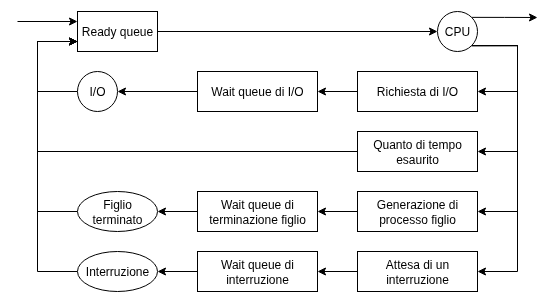
\includegraphics[width=1\linewidth]{Images/processScheduling_enqueueDiagram.png}
	\caption{Diagramma di accodamento per lo scheduling}
\end{figure}

\noindent Come già detto, i processi si spostano tra le varie code disponibili frequentemente; alcuni sistemi operativi, per ridurre il grado di multiprogrammazione, implementano un algoritmo intermedio nello scheduling per rimuovere forzatamente i processi dalla CPU, detto \textbf{avvicendamento dei processi in memoria}.\par
Viene quindi salvato lo stato al momento dello stop del processo rimosso, per poi riprendere da dove è stato interrotto quando lo si reinserisce in memoria. Inoltre, se è implementato lo \textbf{swapping}, i processi si possono spostare dalla memoria centrale al disco per un ulteriore risparmio di spazio. Il salvataggio e ripristino dello stato della CPU si dice invece \textbf{cambio di contesto} e il tempo necessario per attuarlo varia in base alla velocità dell'architettura.\newline
\begin{figure}[h]
	\centering
	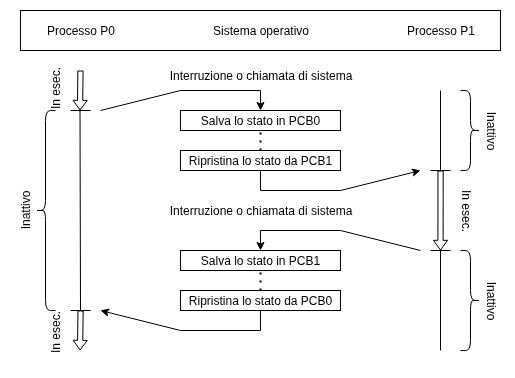
\includegraphics[width=0.9\linewidth]{Images/contextSwitch.png}
	\caption{Diagramma di cambio di contesto}
\end{figure}

\noindent Nella maggior parte dei sistemi operativi i processi lavorano concorrentemente. Si ritiene dunque necessario fornire un meccanismo per la loro creazione e terminazione. I processi genitori possono crearne di figli, i quali a loro volta possono crearne altri. Ciò forma un albero di processi. Per poterli distinguere, i sistemi operativi come Linux li identificano tramite un \textbf{identificatore di processo} (pid), un valore numerico intero univoco per ogni processo.\par
\noindent Generalmente, la creazione di un processo implica l'impiego di determinate risorse: ciò vale sia per genitori che figli. Questi ultimi, in particolare, possono riceverle direttamente dal sistema operativo oppure da un insieme ristretto del genitore. Quest'ultima opzione risulta preferibile in quanto limitando le risorse di un figlio si può evitare che il processo sovraccarichi il sistema usando troppa memoria.\par
Oltre alle varie risorse fisiche e logiche, il genitore può passare ai figli dei dati di inizializzazione, non dissimilmente da una chiamata a funzione. Possiamo avere le seguenti istanze: \begin{itemize}
	\item Il genitore continua l'esecuzione concorrentemente al figlio.
	\item Il genitore attende la terminazione di alcuni o tutti i processi figli.
\end{itemize}
\noindent Inoltre, ci sono due possibilità per quanto riguarda lo spazio di indirizzi del figlio: \begin{itemize}
	\item Il figlio è un duplicato del genitore e ha stessi dati e programma.
	\item Nel figlio si carica un nuovo programma.
\end{itemize}
\noindent Prendiamo come esempio il workflow di UNIX, dove i nuovi processi sono identificati con un pid, generati con fork() e composti da una copia dello spazio di indirizzi del genitore. Ciò consente una facile comunicazione tra genitore e figlio.\par
Entrambi i processi continuano la loro esecuzione all'istruzione successiva al fork(), il quale riporta il valore zero nel nuovo processo, ma ritorna il pid del figlio al genitore, per identificarlo. In genere, dopo la fork(), uno dei due processi impiega una exec() per sostituire lo spazio di memoria del processo con un nuovo programma. La chiamata carica in memoria un file binario cancellando l'immagine di memoria del programma che la contiene e avvia la sua esecuzione. Così i due processi possono comunicare e procedere in modi diversi.\par
Il genitore può, come detto prima, generare più figli o aspettare la loro terminazione invocando wait(). La sua chiamata consente di rimuovere sé stesso dalla coda dei processi pronti fino alla terminazione del figlio. Inoltre, siccome exec() sovrappone lo spazio di indirizzi del processo con un nuovo programma, non può restituire il controllo a meno che non si verifichi un errore. Usando la chiamata execlp(), il figlio sovrappone il proprio spazio di indirizzi con una stringa, per esempio execlp("/bin/ls"), ovvero il comando per ottenere l'elenco dei file in una directory. Quando un processo figlio termina, chiamando implicitamente o esplicitamente exit(), il genitore chiude la fase di attesa data da wait() e termina a sua volta con exit().\newline

\noindent Un processo termina quando è stata eseguita la sua ultima istruzione e inoltra la richiesta di terminazione al sistema operativo con exit().
Se è un figlio, riporta un'informazione di stato al genitore se ha invocato wait(). Tutte le risorse del processo saranno ora liberate dal sistema operativo.
I processi possono essere terminati anche per altre ragioni, come un'interruzione, chiamabile solo dal padre, il quale deve necessariamente conoscere il pid del figlio per poterlo terminare. Generalmente, un genitore può porre fine alla vita di un figlio per svariati motivi, tra cui: \begin{itemize}
	\item Il figlio ha ecceduto nell'uso delle risorse.
	\item Il compito assegnato al figlio è terminato.
	\item Il genitore termina la propria esecuzione. In particolare, i processi terminati il cui padre è ancora attivo sono detti \textbf{zombie}, mentre se il padre termina senza invocare wait(), i figli saranno adottati da systemd per la chiusura e si dicono \textbf{orfani}.
\end{itemize}
\noindent Se un processo termina, così dovranno fare anche gli eventuali figli: questo meccanismo è detto \textbf{terminazione a cascata} ed è una procedura avviata dal sistema operativo. Non è tuttavia comune a tutti i sistemi operativi.\par
La terminazione fornisce uno stato di uscita, dove lo 0 indica una terminazione normale, mentre altri valori segnalano terminazioni anomale. Segue la deallocazione delle risorse utilizzate per il processo.

%

\section{Comunicazione tra processi}
- comunicazione tra processi
- comunicazione a memoria condivisa
- comunicazione a scambio messaggi

%

\section{Architettura client-server}
- architettura client-server